\chapter{Short-cutting heuristics}


\section{Simple Heuristic}
\begin{enumerate}
    \item {The order of appearance of points in the hamiltonian cycle is the order of their appearance in the Euler tour. (For each of the points, we retain the first occurence of the point and discard the remaining).}
    % \item Remove repeated points in the Euler tour to get a Hamiltonian cycle.
    \item Time complexity is $O(n)$.
\end{enumerate}
% \includegraphics[scale=0.5]{simple.png}

\section{Tri-Opt Heuristic}

\begin{enumerate}
    \item In this heuristic we take a Euler tour and greedily remove the repeated vertices which have higher heuristic value.
    \item The heuristic value used is sum of distances from the vertex to adjacent vertices minus distance between the adjacent vertices.
    \item We can see that this is better than previous one but we are performing it on a Euler tour, hence there is still room for imprevement.
    \item Time complexity is $O(n)$.
\end{enumerate}
% \includegraphics[scale=0.5]{simple.png}



\section{Tri-Comp Heuristic}

\begin{enumerate}
    \item This heuristic is applied on Multi graph (H) instead of one Euler tour.
    \item Here we start with vertices of order greater than two and greedily remove its edges until its order is two.
    \item The idea is that in the final hamiltonian cycle which we need to arrive by short cutting has degree two for all the vertices.
    \item Two things we need to do are - pair up the free vertices formed greedily and make sure the process does not result in two disjoint components
    \item The heuristic value here is sum of distances between paired up vertices and distace of two edges that remained with our vertex.
    \item Since our problem is in 2d space, each vertex in MST will have a degree of maximum 5, so our multi graph will have a maximum degree of 6. This property highly affect the theoritical complexity of our heuristic.
    \item Time complexity for checking the graph connectivity is $O(n)$ and therefore, time complexity for the tri-compt heuristic is $O(n^2)$.
\end{enumerate}
% \includegraphics[scale=0.5]{simple.png}

\section{DIH-Tri-Comp Heuristic}
\begin{figure}[h]
    \centering
    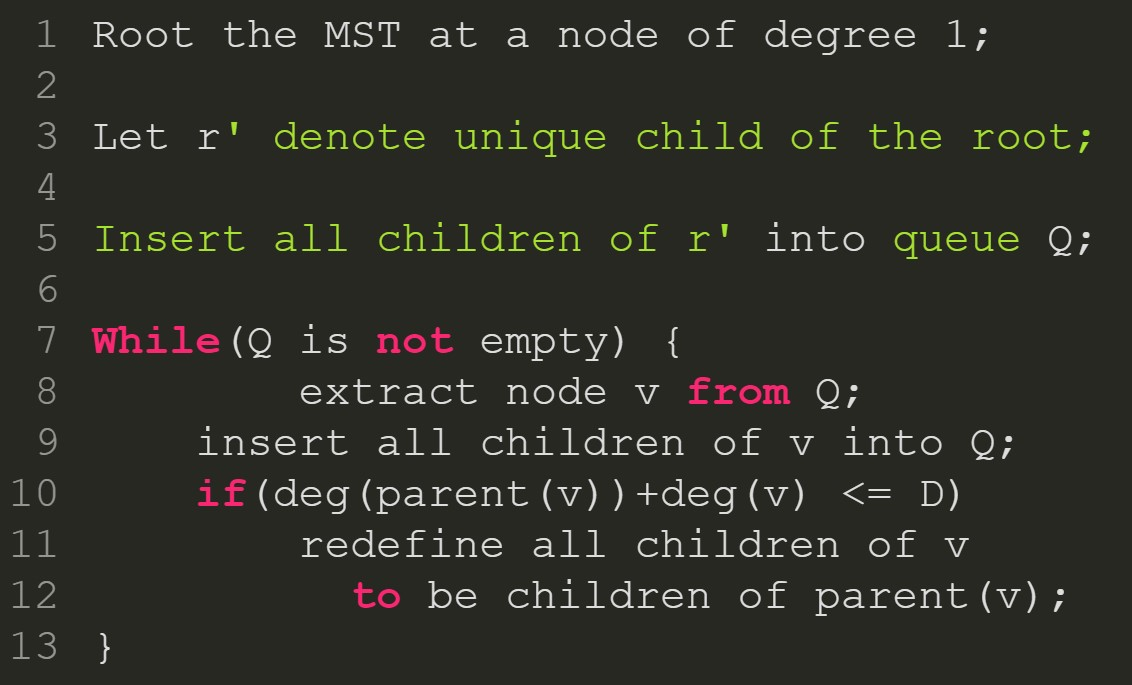
\includegraphics[scale=0.3]{5.jpg}
    \caption{Pseudo code for DIH heuristic}
\end{figure}
\begin{figure}[h]
    \centering
    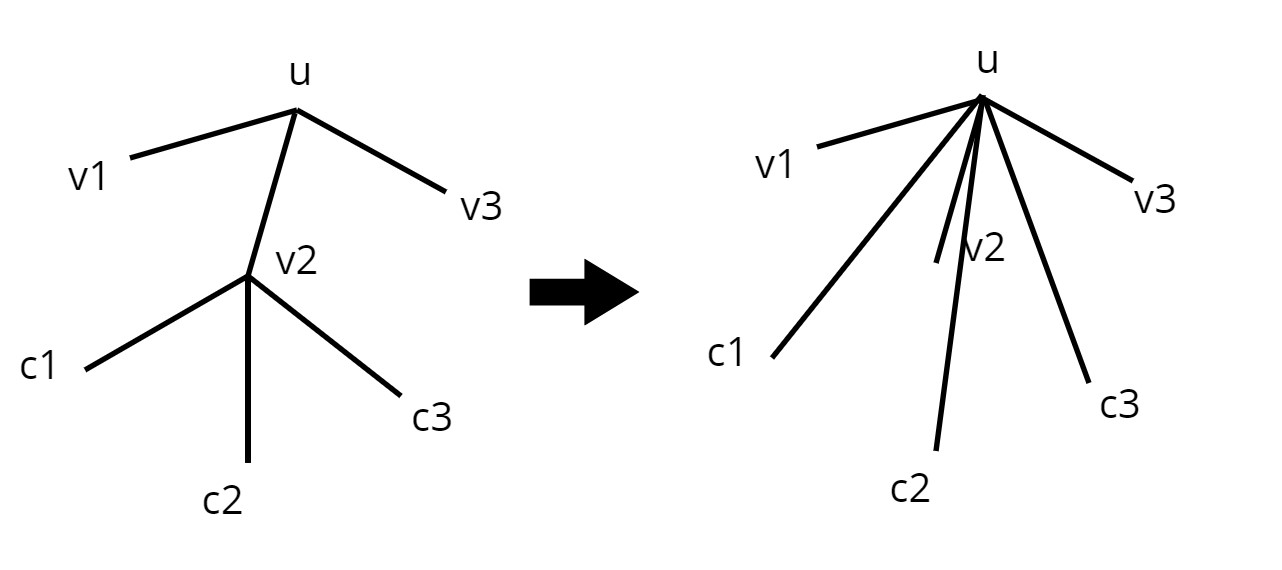
\includegraphics[scale=0.3]{4.jpg}
    \caption{Applying DIH on $T$(left) to get $T'$(right)}
\end{figure}
\begin{enumerate}
    \item This heuristic is DIH(Degree Increasing Heuristic) optimization applied on the MST $T$ to get a new tree $T'$, then creating a multigraph $H'$ from $T'$, followed by applying Tri-compt heuristic on the multigraph $H'$.
    \item We want to increase the order of a vertex in MST by adding the vertices  of its children to itself
    \item We can see that the tree $T'$ is no longer MST but this process preserves the Euler tours i.e. the set of Euler tours of this tree $T'$ is super set of that of the MST $T$.
    \item This way we are applying heuristic on a bigger space than that of the former one and might have a chance of getting better results.
    \item  DIH can be implemented with $O(n)$, so comp heuristic is the bottleneck here. Overall time complexity is $O(n^2)$
\end{enumerate}
\vspace{7in}
\section{Performance analysis of heuristics}

We measured the performance of the four heuristics over 100 TSP problems from TSPLIB which is a library of sample instances for the TSP (and related problems) from various sources and of various types.

\begin{figure}[h]
    \centering
    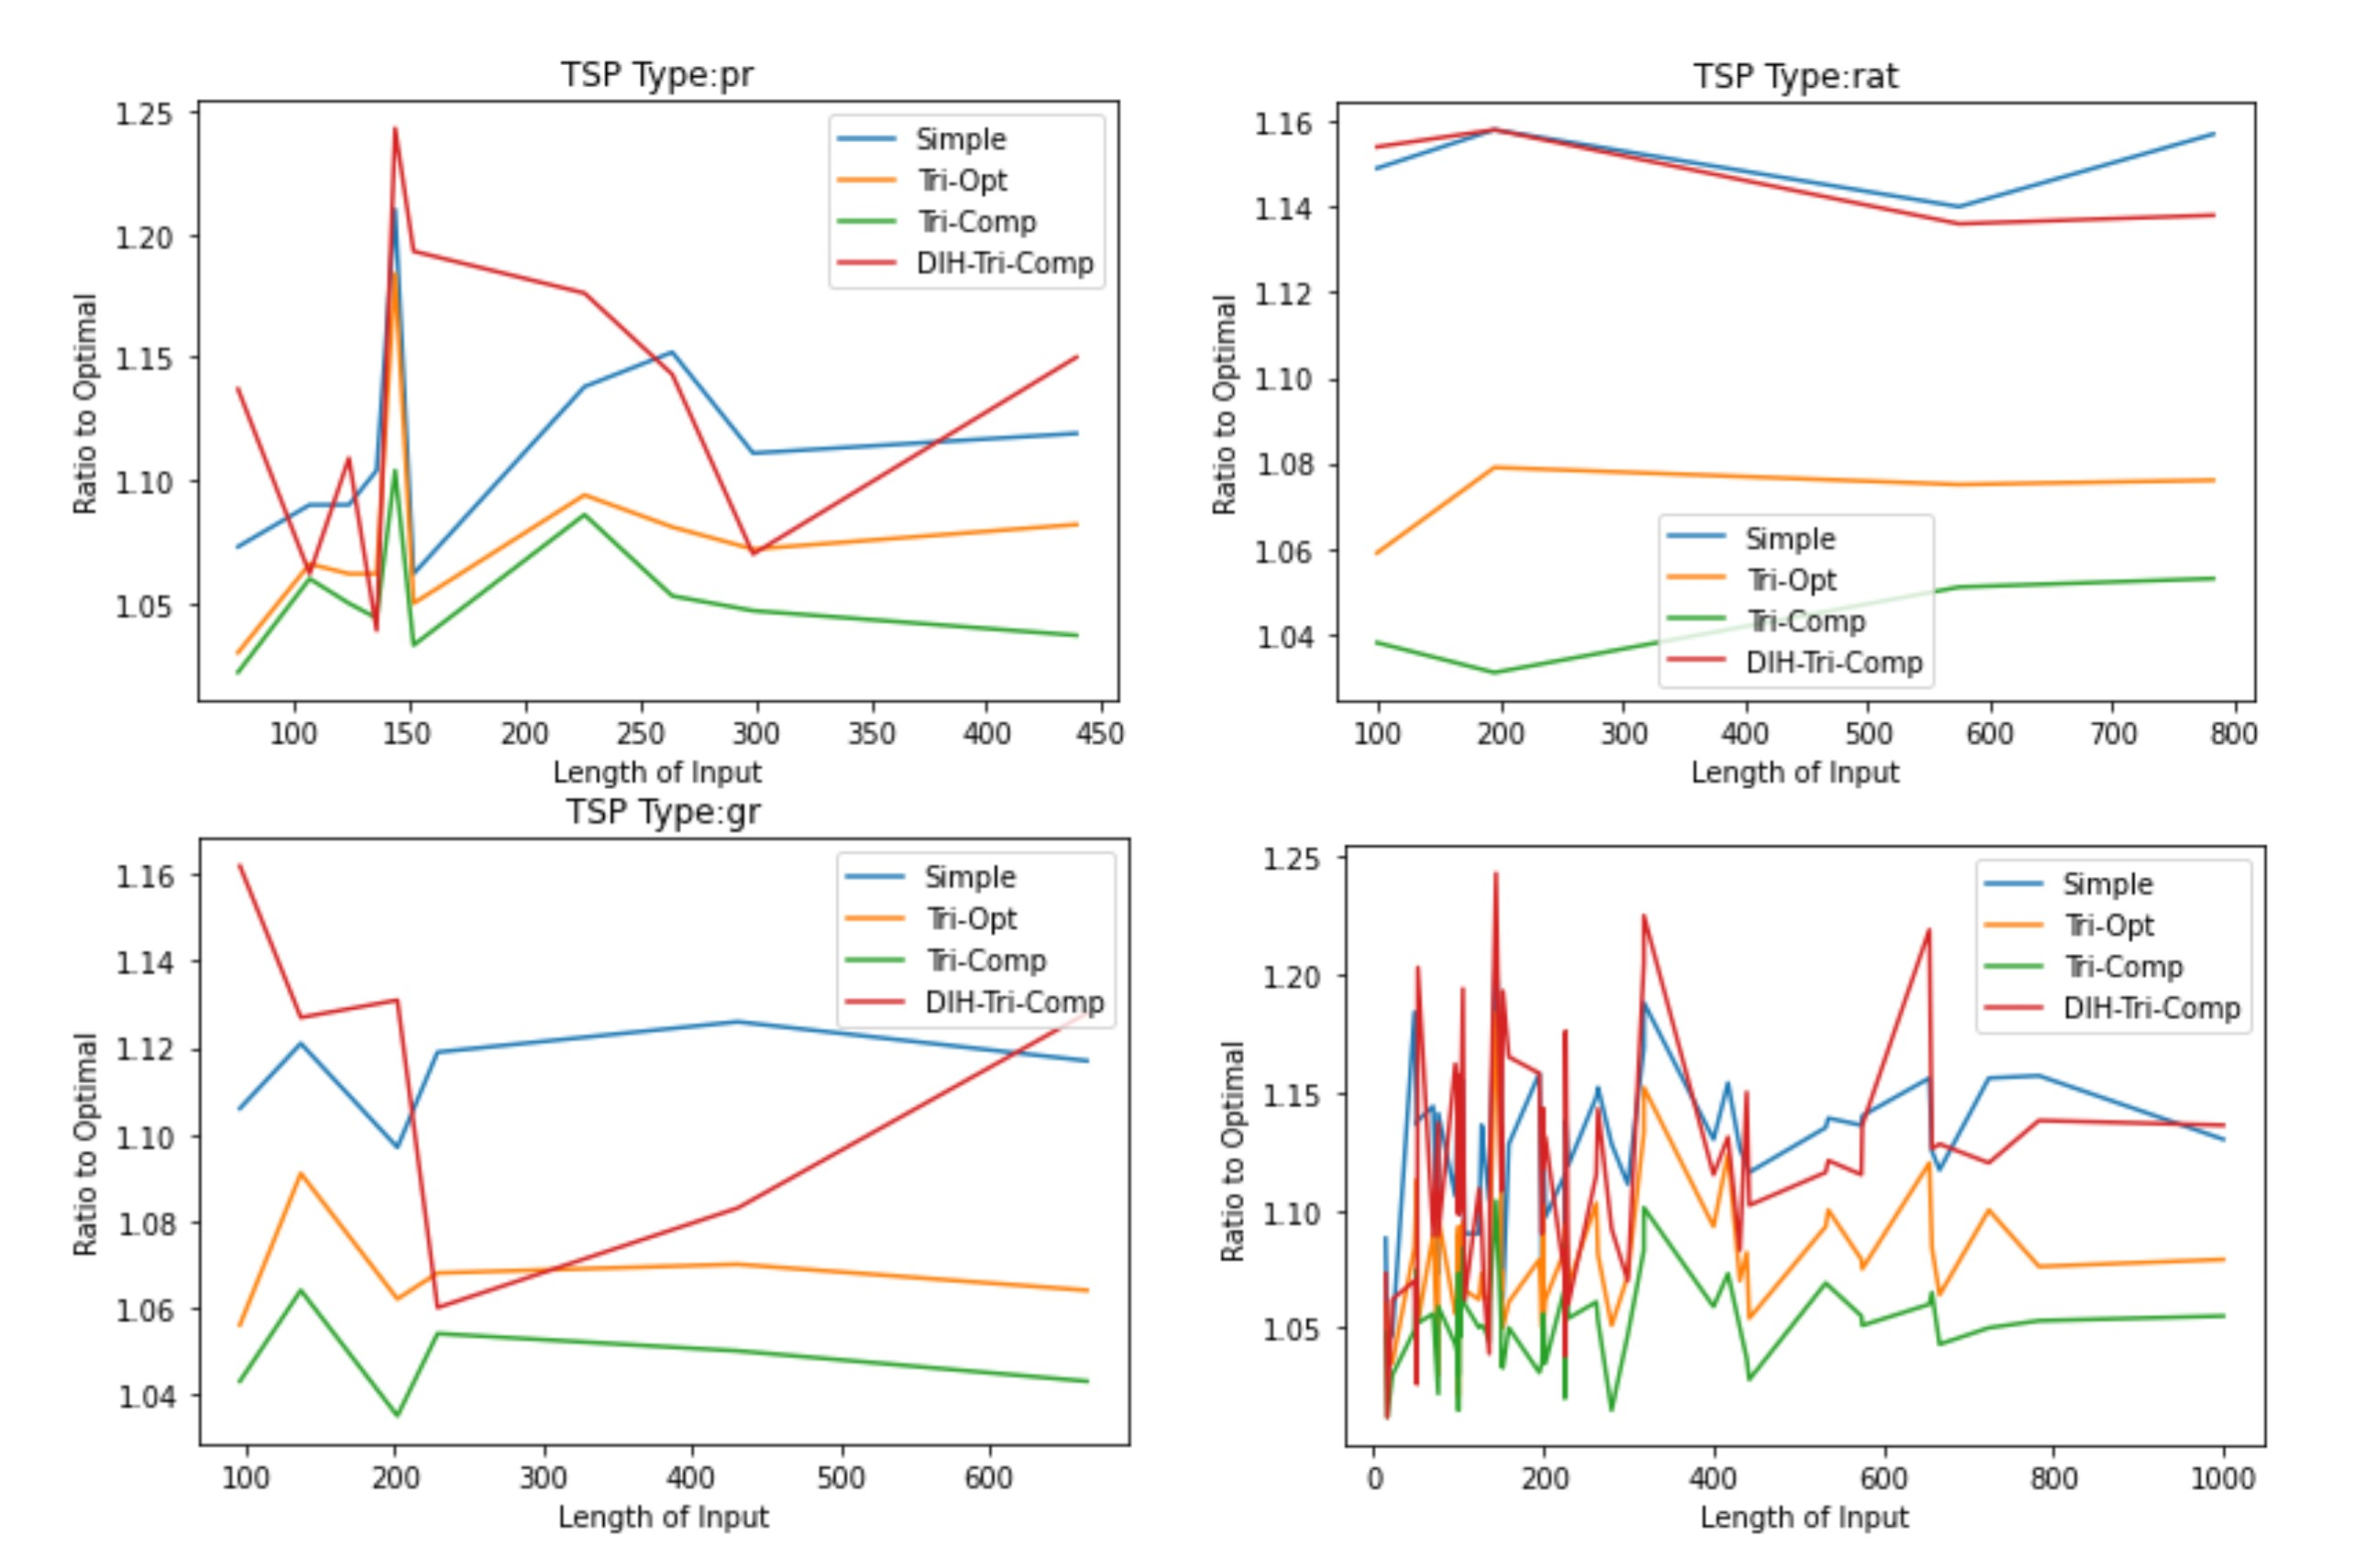
\includegraphics[scale=0.22]{6.jpg}
    \caption{Performance of heuristics on different families of datasets}
\end{figure}